\chapter{Összegzés}

A streaming rendszereket kiszolgáló technológiák fejlődése közel sem ért véget, a QUIC protokoll -- és az arra épülő Media over QUIC\cite{ietf-moq-transport-11} (MoQ) -- előretörésével, új modern CDN-funkcionalitásokkal\cite{openconnect}, a szerverfarmokban használt alkalmazásspecifikus chipek fejlődésével, illetve hatékonyabb kodekek megjelenésével egyre magasabb minőséget lehet szolgáltatni. Az általam bemutatott rendszer egy egyszerűsített példája a streaming rendszereknek, amely lehetőséget ad arra, hogy megértsük a mögöttes technológiákat és azok működését, betekintést nyújt néhány tipikusan streamingre használt AWS-erőforrás világába, a~tervezési technikák palettájába.

A fejlesztés ideje alatt ahogy egyre több erőforrást kötöttem be, nőtt a felhőszolgáltatások költsége is. A dolgozat írásákor többször teszteltem a megoldást, a~márciusi összköltsége \$67.98 lett, áprilisban \$73.29 (lásd \refstruc{fig:costs}). Ezekben az összegekben a~legjelentősebbek közé tartozott az RDS-adatbázisnak, az ALB-példánynak, a MediaLive futtatásának és az ECS-klaszternek a költsége, ezek nem on-demand jellegűek, VM van mögöttük. Pár szolgáltatás (Lambda, CloudWatch Logs) pedig a \emph{free tier}, azaz ingyenes átkategóriában tudott maradni. Májusra \$78-t jelzett előre, a hónapban végzett k6 tesztelés alatti (\ref{sec:vod_test}. alfejezet) kb. 100 GB CDN-forgalom se emelte jobban.

\begin{figure}[h]
  \centering
  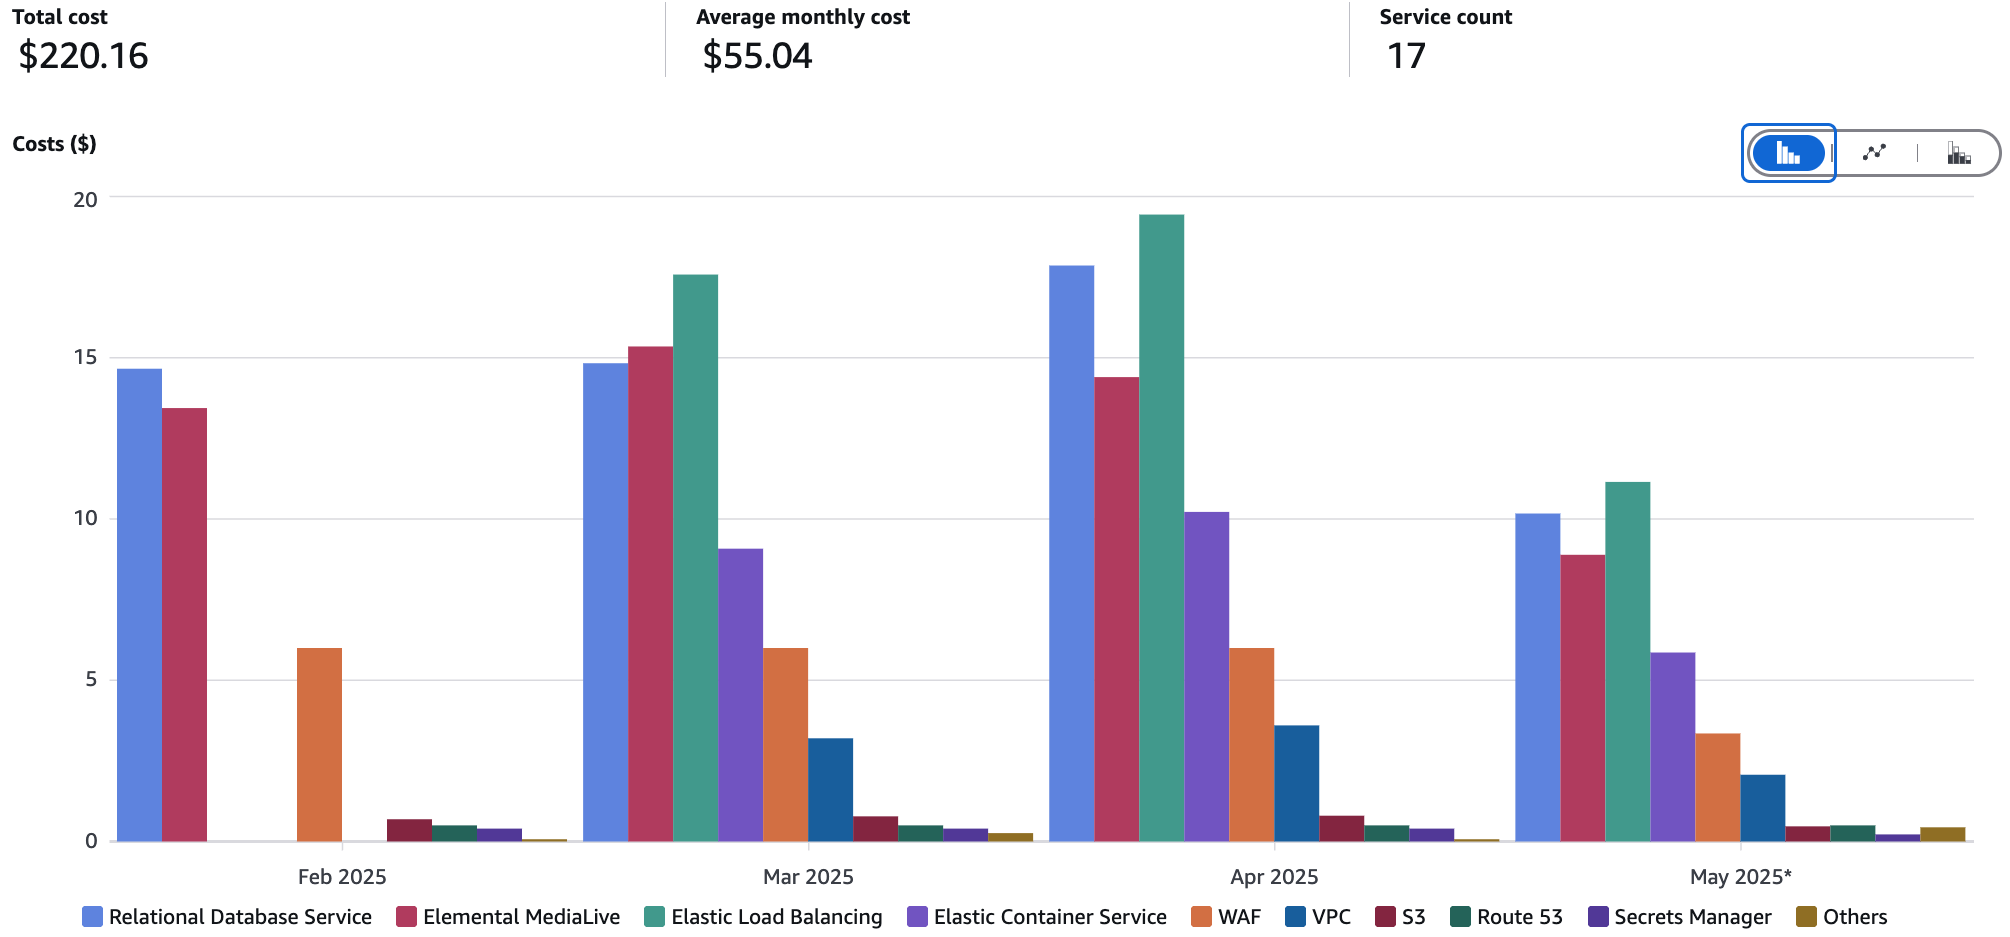
\includegraphics[width=150mm, keepaspectratio]{figures/costs.png}
  \caption{Költségkimutatás az AWS-konzolon.}
  \label{fig:costs}
\end{figure}

\section{Továbbfejlesztés lehetőségei}

Architekturális szempontból a webszerver átszervezhető mikroszolgáltatásos alapokra, amennyiben a jövőben a rendszer bővítése, új funkciók bevezetése indokolttá teszi, ezzel is jobban támogatva a már megkezdett event-driven architecture (EDA)\cite{eda} irányvonalat.

Biztonság szempontjából a rendszer továbbfejlesztése érdekében érdemes lenne megfontolni a naplózást kiterjeszteni a CDN és a WAF szintjén ``access loggingra'' is, a VPC-n belül a Flow logok bekapcsolására. Élő, nagy forgalmú rendszerben kihagyhatatlan kötelességünk volna a WAF ACL-ben foglalt szabályokat finomhangolni veszélyes forgalom kiszűrésére. \Az+\ref{sec:vpc}.~alfejezetben említett NAT Gateway és VPC Endpoint megoldások alkalmazása is javallott volna.

A kiszolgálás minőségének javítására érdemes lehet akár a CloudFront-disztribúció cache beállításait is optimalizálás szempontjából újraszemlézni. Felmerülhet egy nagyobb rendszernél a webszerver felé irányított forgalom hálózati terheléséből származó kihívásokra felkészíteni az ALB-példányt is, erre lehet igénybe venni Load balancer Capacity Unit (LCU) foglalást, amely biztosít megfelelő számítási kapacitást a forgalom fogadására. Emellett az ECS-klaszterbe is be lehet vezetni egy automatikus skálázási megoldást, amely a forgalom növekedésével automatikusan új taszkokat indít el az ECS-szolgáltatásban, ezzel biztosítva a megfelelő számítási kapacitást.

A rendszer erős kódmigrálást, infrastruktúra-átalakítást igényelne, amennyiben cél volna a \emph{vendor lock-in}\cite{lockIn} kockázatainak mitigálása. Ehhez javasolt lenne a Kubernetesre\footnote{\url{https://kubernetes.io/}} való áttérés ECS-ről\cite{k8s}, Ceph\footnote{\url{https://ceph.io/en/}} használata S3 helyett, a Kubernetes alá hozható az~adatbázis, illetve a Lambda-függvények is kis mikroszolgáltatások formájában. A~MediaConvert, a~MediaLive és MediaPackage szolgáltatások kiváltása már bonyolultabb lehet, ebben segíthet az általam korábbi projektben megismert FFMpeg és az NGINX RTMP\leavevmode\hbox{-}modulja\cite{rtmpNginx}, ahogy azt \az+\ref{sec:elso_lepesek} alfejezetben is említettem.

Nem utolsó sorban a live streaming kiterjesztése még egy feladat, ami várat magára. A rendszer jelenleg nem engedi több élő adás indítását, ezt lehetne kiterjeszteni kódból történő dinamikus MediaLive- és MediaPackage-csatornák felkonfigurálására.
